\documentclass[aspectratio=169]{beamer}
\mode<presentation>
{
  \usetheme{metropolis}      % or try Darmstadt, Madrid, Warsaw, ...
  \usecolortheme{default} % or try albatross, beaver, crane, ...
  \usefonttheme{structurebold}  % or try serif, structurebold, ...
  \setbeamercolor{background canvas}{bg=white}
  \setbeamertemplate{navigation symbols}{}
  \setbeamertemplate{bibliography item}{\insertbiblabel}
  %\setbeamertemplate{caption}[numbered]
} 
\usepackage[english]{babel}
\usepackage[utf8x]{inputenc}
\usepackage{listings}             % Include the listings-package
\usepackage{bm}	% math package
\hypersetup{
    colorlinks = true,
    linkcolor = {black},
    urlcolor = {blue}
}

\DeclareMathOperator*{\argmin}{arg\,min}

\title[Deep Learning and Temporal Data Processing]{Deep Learning and Temporal Data Processing}
\subtitle{1 - Deep Neural Networks}
\institute{University of Modena and Reggio Emilia}
\author{Andrea Palazzi}
\date{June 21th, 2017}

\setbeamertemplate{caption}{\raggedright\insertcaption\par}

\def\thisframelogos{}

\newcommand{\framelogo}[1]{\def\thisframelogos{#1}}
\newcommand{\R}{\mathbb{R}}

\addtobeamertemplate{frametitle}{}{%
\begin{tikzpicture}[remember picture,overlay]
\node[anchor=north east] at (current page.north east) {%
    \foreach \img in \thisframelogos {%
        %\hspace{.5ex}%
        \includegraphics[height=3.5ex]{\img}%
    }%
};
\end{tikzpicture}}

\begin{document}

\framelogo{img/template/logo_unimore_white.png}

\bgroup
\renewcommand{\insertframenumber}{}
\begin{frame}[noframenumbering]
  \titlepage
\end{frame}
\egroup
\begin{frame}{Agenda}
  \tableofcontents
\end{frame}


%%%%%%%%%%%%%%%%%%%%%%%%%%%%%%%%%%%%%%%%%%%%%%%%%%%%%%%%%%%%%%%%%%
%%%%%%%%%%%%%%%%%%%%%%%%%%%%%%%%%%%%%%%%%%%%%%%%%%%%%%%%%%%%%%%%%%
%%%%%%%%%%%%%%%%%%%%%%%%%%%%%%%%%%%%%%%%%%%%%%%%%%%%%%%%%%%%%%%%%%

\section{Introduction}

%%%%%%%%%%%%%%%%%%%%%%%%%%%%%%%%%%%%%%%%%%%%%%%%%%%%%%%%%%%%%%%%%%

\begin{frame}{Here is the Hype}
\begin{figure}
\begin{tabular}{c}
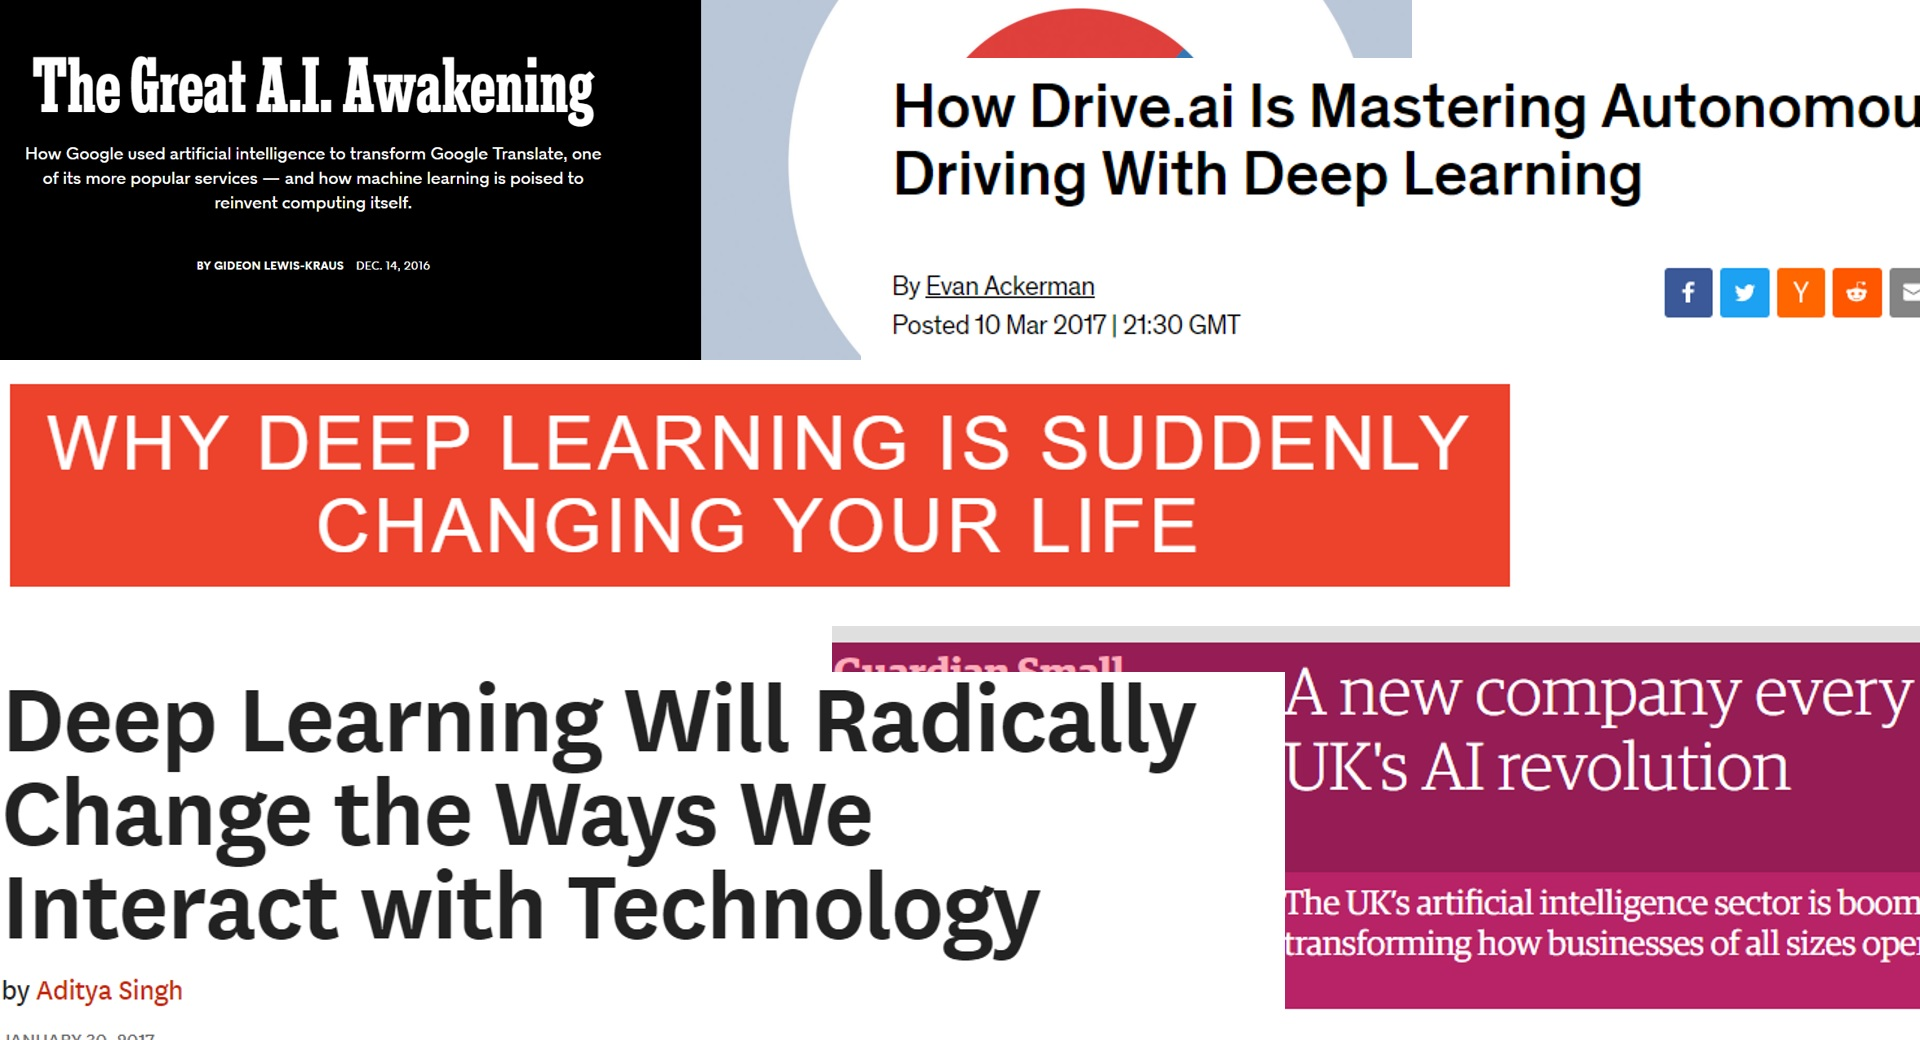
\includegraphics[width=0.9\textwidth]{img/dnn/deep_learning_media.jpg}
\end{tabular}
\end{figure}
\end{frame}

%%%%%%%%%%%%%%%%%%%%%%%%%%%%%%%%%%%%%%%%%%%%%%%%%%%%%%%%%%%%%%%%%%
%%%%%%%%%%%%%%%%%%%%%%%%%%%%%%%%%%%%%%%%%%%%%%%%%%%%%%%%%%%%%%%%%%
%%%%%%%%%%%%%%%%%%%%%%%%%%%%%%%%%%%%%%%%%%%%%%%%%%%%%%%%%%%%%%%%%%

\section*{How did we get there?}

%%%%%%%%%%%%%%%%%%%%%%%%%%%%%%%%%%%%%%%%%%%%%%%%%%%%%%%%%%%%%%%%%%

\begin{frame}{Neural Networks are NOT new}
Despite the current hype on the deep learning revolution, neural networks algorithms are far from being new. This is the \textbf{third time} that neural networks come to the fore:
\begin{itemize}
\item \textbf{1940s-1960s}: theories of biological inspired learning\cite{morris1999hebb,mcculloch1943logical}. The first pioneering models such as the perceptron \cite{rosenblatt1958perceptron}. A single neuron is trained for the first time.
\item \textbf{1980s-1990s}: neural networks with a couple of hidden layers are trained by means of backpropagation\cite{rumelhart1988learning}.
\item \textbf{2006-now}: current wave of research.
\end{itemize}
\end{frame}

%%%%%%%%%%%%%%%%%%%%%%%%%%%%%%%%%%%%%%%%%%%%%%%%%%%%%%%%%%%%%%%%%%

\begin{frame}{Why Now?}
Despite underlying ideas of deep learning have been around since a while, only recently performance boosted. This is due to a variety of complementary factors:
\begin{itemize}
\item large labeled datasets
\item computational power
\item training on GPUs (eventually distributed)
\item ...
\end{itemize}

\end{frame}

%%%%%%%%%%%%%%%%%%%%%%%%%%%%%%%%%%%%%%%%%%%%%%%%%%%%%%%%%%%%%%%%%%

\begin{frame}{2003: Large Dataset}
\begin{figure}
\begin{tabular}{c}
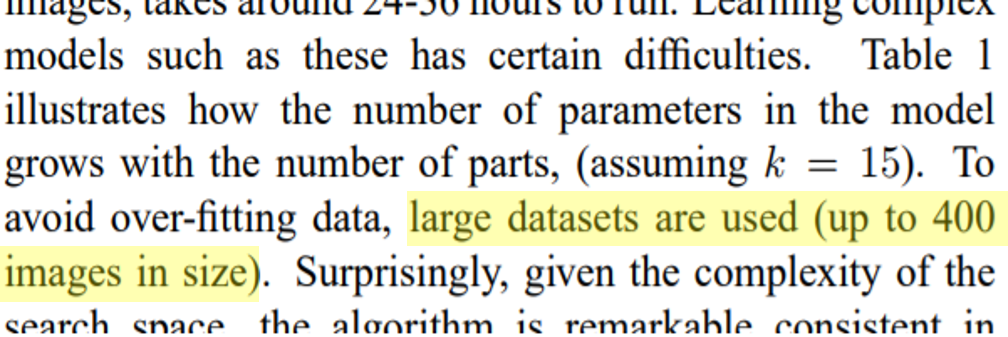
\includegraphics[width=0.7\textwidth]{img/dnn/2003_large_dataset.png}\\
\end{tabular}
\vspace{0.5cm}
\caption{Fergus, Robert, Pietro Perona, and Andrew Zisserman. "Object class recognition by unsupervised scale-invariant learning." Computer Vision and Pattern Recognition, 2003. Proceedings. 2003 IEEE Computer Society Conference on. Vol. 2. IEEE, 2003.}
\end{figure}
\end{frame}

%%%%%%%%%%%%%%%%%%%%%%%%%%%%%%%%%%%%%%%%%%%%%%%%%%%%%%%%%%%%%%%%%%

\begin{frame}{2017: Large Dataset}
\begin{figure}
\begin{tabular}{c}
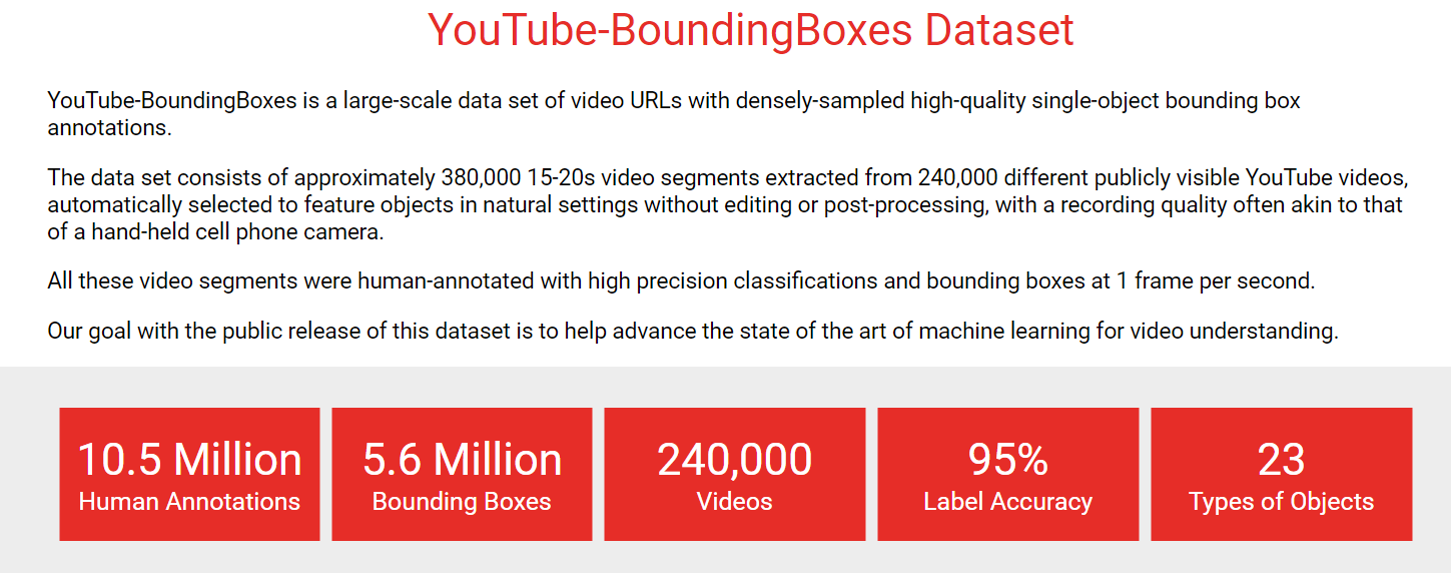
\includegraphics[width=0.85\textwidth]{img/dnn/2017_large_dataset.png}\\
\end{tabular}
\vspace{0.5cm}
\caption{Real, Esteban, et al. "YouTube-BoundingBoxes: A Large High-Precision Human-Annotated Data Set for Object Detection in Video." arXiv preprint arXiv:1702.00824 (2017).}
\end{figure}
\end{frame}

%%%%%%%%%%%%%%%%%%%%%%%%%%%%%%%%%%%%%%%%%%%%%%%%%%%%%%%%%%%%%%%%%%

\begin{frame}{Why Size Matters}
\begin{figure}
\begin{tabular}{c}
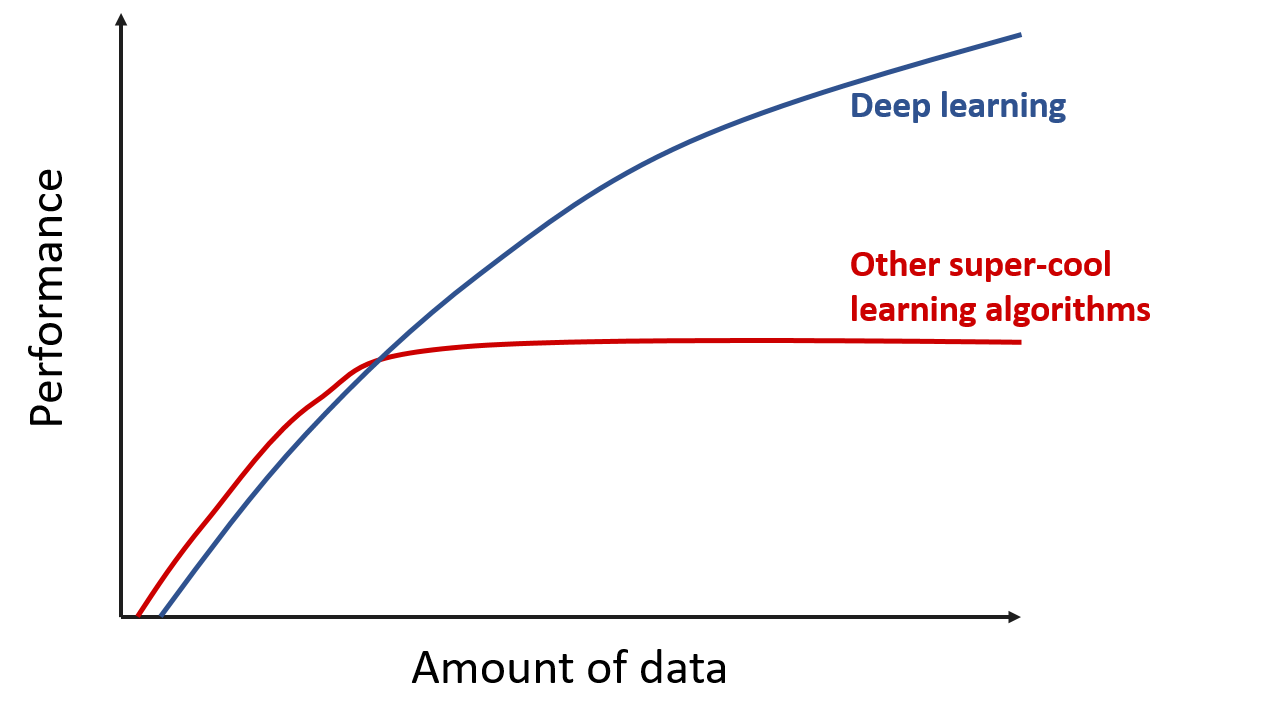
\includegraphics[width=0.7\textwidth]{img/dnn/deep_learning_scale.png}
\end{tabular}
\caption{Andrew Ng. "What data scientists should know about deep learning".}
\end{figure}
\end{frame}

%%%%%%%%%%%%%%%%%%%%%%%%%%%%%%%%%%%%%%%%%%%%%%%%%%%%%%%%%%%%%%%%%%

\begin{frame}{The Challenge of Data Representation}
Performance of machine learning algorithms heavily depends on the way we represent the data. These discrete pieces of information that we use as a proxy to model the complexity of the world are usually called \textbf{features}.\\
\vspace{0.5cm}
Generally speaking, for a long time, these features have been \textbf{handcrafted} differently for each task at hand.\\
\vspace{0.5cm}
Conversely, deep learning algorithms allow to \textbf{learn the right representation directly from the data}.
\end{frame}

%%%%%%%%%%%%%%%%%%%%%%%%%%%%%%%%%%%%%%%%%%%%%%%%%%%%%%%%%%%%%%%%%%
%%%%%%%%%%%%%%%%%%%%%%%%%%%%%%%%%%%%%%%%%%%%%%%%%%%%%%%%%%%%%%%%%%
%%%%%%%%%%%%%%%%%%%%%%%%%%%%%%%%%%%%%%%%%%%%%%%%%%%%%%%%%%%%%%%%%%

\section{One step back: Linear classifiers}

\begin{frame}{Linear Classifier}
For the purpose of this lecture, we'll stick to the task of image classification.\\
Let's assume we have a training dataset of $N$ images
\begin{equation*}
x_i \in \R^D, i = 1, \dots, N
\end{equation*}
that we want to classify into $K$ distinct classes.\\
Thus, training set is made by couples:
\begin{equation*}
(x_i, y_i),\ where \, y_i \in \{1, \dots, K\}
\end{equation*}
Our goal is to define a function $f: \R^D \mapsto \R^K$ that maps images to class scores.
\end{frame}

%%%%%%%%%%%%%%%%%%%%%%%%%%%%%%%%%%%%%%%%%%%%%%%%%%%%%%%%%%%%%%%%%%

\begin{frame}{Linear Classifier}
Making a real-world example: let's take the \texttt{CIFAR-10} dataset, which consists of $N=60000$ 32x32 RGB images belonging to 10 different classes.\\
\begin{figure}
\begin{tabular}{c}
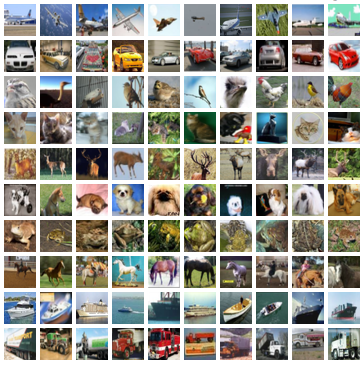
\includegraphics[width=0.4\textwidth]{img/dnn/cifar10.png}
\end{tabular}
\end{figure}
\end{frame}

%%%%%%%%%%%%%%%%%%%%%%%%%%%%%%%%%%%%%%%%%%%%%%%%%%%%%%%%%%%%%%%%%%

\begin{frame}{Linear Classifier}
Each image is $32$x$32$x$3$, thus it can be thought as a column vector $x_i \in \R^{3072}$.\\
Now we can define a \textbf{linear mapping}:
\begin{equation*}
f(x_i,W,b) = Wx_i + b
\end{equation*}
where the parameters are:
\begin{itemize}
\item the weight matrix $W \in \R^{10 x 3072}$ 
\item the bias vector $b \in \R^{10}$.
\end{itemize}
\small{Intuitively, our goal is to learn the parameters from the training set \emph{s.t.} when a new test image $x^{test}_i$ is given as input, the score of the correct class is higher that the scores of other classes.}
\end{frame}

%%%%%%%%%%%%%%%%%%%%%%%%%%%%%%%%%%%%%%%%%%%%%%%%%%%%%%%%%%%%%%%%%%\\

\begin{frame}{Linear Classifier}
\begin{figure}
\begin{tabular}{c}
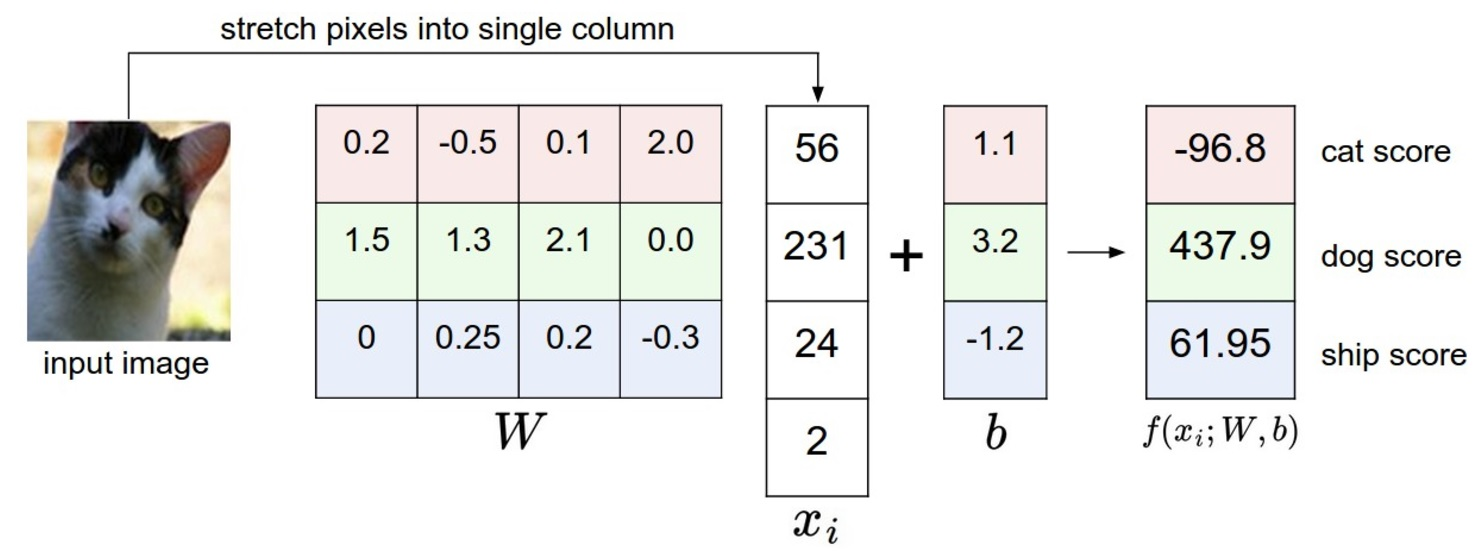
\includegraphics[width=0.8\textwidth]{img/dnn/linear_classifier.jpg}
\end{tabular}
\end{figure}
\small{Example of mapping an image to a score. For the sake of visualization, here the image is assumed to have only 4 grayscale pixels.}
\end{frame}

%%%%%%%%%%%%%%%%%%%%%%%%%%%%%%%%%%%%%%%%%%%%%%%%%%%%%%%%%%%%%%%%%%\\

\begin{frame}{Logistic Regression}

\end{frame}

%%%%%%%%%%%%%%%%%%%%%%%%%%%%%%%%%%%%%%%%%%%%%%%%%%%%%%%%%%%%%%%%%%\\

\begin{frame}{Softmax Classifier}
First let's introduce the \textbf{softmax function}:
\begin{equation*}
softmax_j(\textbf{z}) = \frac{e^{z_j}}{\sum_k e^{z_k}}
\end{equation*}
It takes a vector of arbitrary real-valued scores $\textbf{z}$ and squashes it to a vector of values between zero and one that sum to one.\\
\emph{e.g.}
\begin{equation*}
\textbf{z} = \begin{bmatrix}1.2\\5.1\\2.7\end{bmatrix}
\quad softmax(\textbf{z}) = \begin{bmatrix}0.018\\0.90\\0.08\end{bmatrix}
\end{equation*}
\end{frame}

%%%%%%%%%%%%%%%%%%%%%%%%%%%%%%%%%%%%%%%%%%%%%%%%%%%%%%%%%%%%%%%%%%\\

\begin{frame}{Softmax Classifier}
\textbf{Softmax Classifier} generalizes Logistic Regression classifier to multi-class classification.\\
\vspace{0.2cm}
In the Softmax classifier the scores of linear function mapping $f(x_i,W) = Wx_i$ are interpreted as unnormalized log probabilities and we use the \textbf{cross-entropy loss}:
\begin{equation*}
L_i = -log\left(\frac{e^{f_{y_{i}}}}{\sum_j e^{f_{j}}}\right)
\end{equation*}
\small{Prove yourself that this loss function makes sense.}
%Softmax Classifier has the appealing property to produce an easy-to-interpret output, that is the normalized score confidence for each class.

\end{frame}

%%%%%%%%%%%%%%%%%%%%%%%%%%%%%%%%%%%%%%%%%%%%%%%%%%%%%%%%%%%%%%%%%%
%%%%%%%%%%%%%%%%%%%%%%%%%%%%%%%%%%%%%%%%%%%%%%%%%%%%%%%%%%%%%%%%%%
%%%%%%%%%%%%%%%%%%%%%%%%%%%%%%%%%%%%%%%%%%%%%%%%%%%%%%%%%%%%%%%%%%

\section{Modeling a Neuron}

\begin{frame}{Introduction}
Neural Networks are a mathematical model \textbf{coarsely} inspired by the way our own brain works.
\begin{figure}
\begin{tabular}{c}
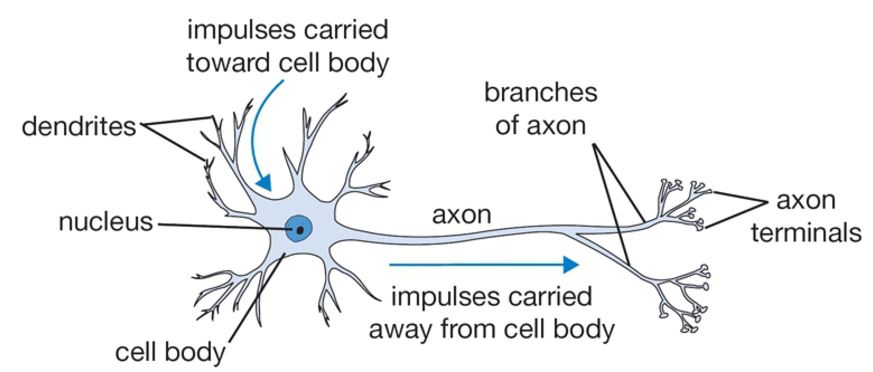
\includegraphics[width=0.4\textwidth]{img/dnn/biological_neuron.jpg}
\end{tabular}
\end{figure}
\small{Neurons are the basic computational unit of our brain. Approximately 86 billion neurons can be found in the human nervous system and they are connected with approximately $10^{14}$ - $10^{15}$ \textbf{synapses}. Each neuron receives input signals from its \textbf{dendrites} and produces output signals along its (single) \textbf{axon}. The axon eventually branches out and connects via synapses to dendrites of other neurons.}
\end{frame}

%%%%%%%%%%%%%%%%%%%%%%%%%%%%%%%%%%%%%%%%%%%%%%%%%%%%%%%%%%%%%%%%%%

\begin{frame}{Modeling a Single Neuron}
More formally, we can model a single \textbf{neuron} as follows:
\begin{figure}
\begin{tabular}{c}
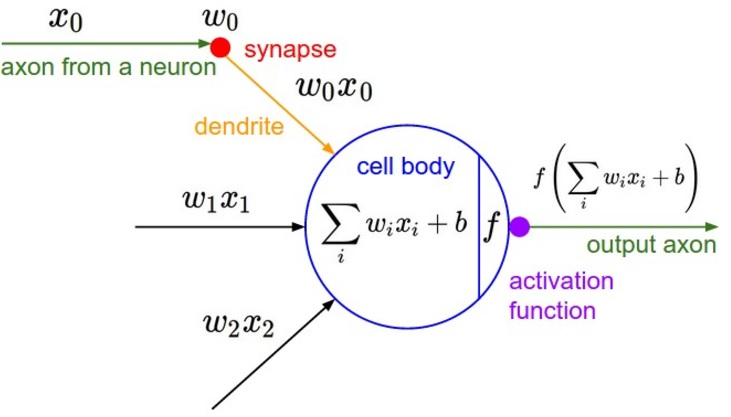
\includegraphics[width=0.4\textwidth]{img/dnn/single_neuron.jpg}
\end{tabular}
\end{figure}
Each neuron can have multiple inputs. The neuron's output is the dot product between the inputs and its weights, plus the bias: then, a non-linearity is applied.
\end{frame}

%%%%%%%%%%%%%%%%%%%%%%%%%%%%%%%%%%%%%%%%%%%%%%%%%%%%%%%%%%%%%%%%%%

\begin{frame}{Modeling a Single Neuron}
It's easy to see that a single neuron can be used to implement a binary classifier.\\
\vspace{1cm}
Indeed, when \textbf{cross-entropy loss} is applied to neuron's output, we can optimize a \textbf{binary Softmax classifier} (\emph{a.k.a.} Logistic regression).
\end{frame}

%%%%%%%%%%%%%%%%%%%%%%%%%%%%%%%%%%%%%%%%%%%%%%%%%%%%%%%%%%%%%%%%%%

\begin{frame}{Neuron Activation}

\textbf{Activation functions} are non-linear functions computed on the output of each neuron.\\
There are a number of different activation functions you could use. In practice, the three most widely used functions have been \textit{sigmoid}, \textit{tanh} and \textit{ReLu}. Nonetheless, more complex activation functions exist (\emph{e.g.} \cite{he2015delving,goodfellow2013maxout}).\\
\vspace{0.8cm}
\begin{columns}
\begin{column}{0.25\textwidth}
\begin{tabular}{c}
\\
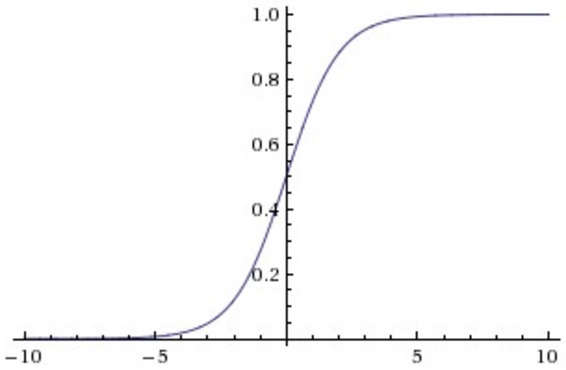
\includegraphics[width=\textwidth]{img/cnn/act_sigmoid.jpg}\\
\end{tabular}
\end{column}
\begin{column}{0.7\textwidth}
\textbf{Sigmoid} nonlinearity has form $\sigma(x) = 1 / (1 + e^{-x})$. Sigmoid function squashes any real-valued input into range $[0, 1]$. It has seen frequent use historically, yet now it's rarely used. It has two major drawbacks:
\begin{itemize}
\item saturates and kill the gradient
\item output is not zero centered
\end{itemize}
\end{column}
\end{columns}
%\textbf{Why do we bother using activations?}\\
%\pause
%Composition of linear functions is a linear function. Without nonlinearities, neural networks would reduce to 1 layer logistic regression.
%\begin{figure}
%\begin{tabular}{ccc}
%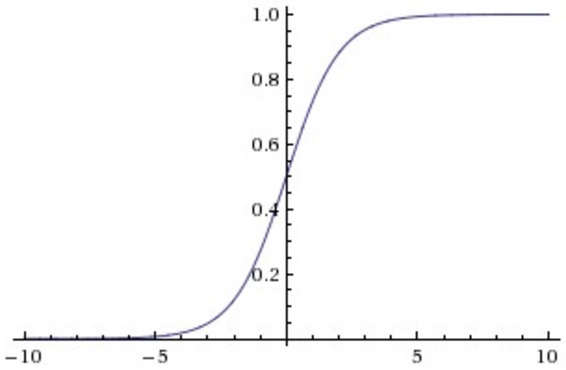
\includegraphics[width=0.3\textwidth]{img/cnn/act_sigmoid.jpg}&
%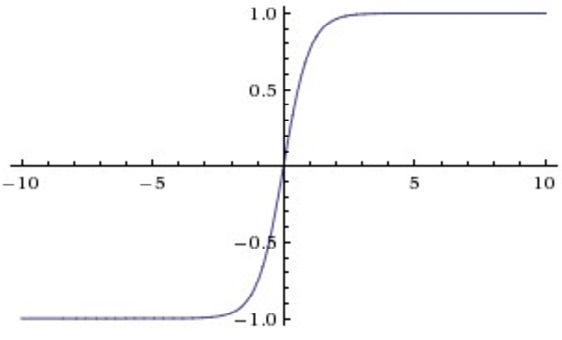
\includegraphics[width=0.3\textwidth]{img/cnn/act_tanh.jpg} & 
%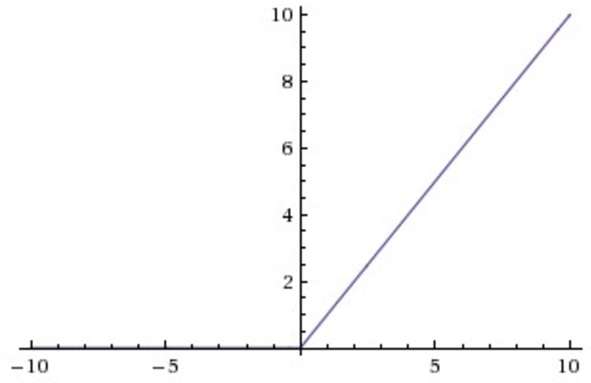
\includegraphics[width=0.3\textwidth]{img/cnn/act_relu.jpg}\\
%Sigmoid & Tanh & ReLu
%\end{tabular}
%\end{figure}
\end{frame}

%%%%%%%%%%%%%%%%%%%%%%%%%%%%%%%%%%%%%%%%%%%%%%%%%%%%%%%%%%%%%%%%%%

\begin{frame}{Neuron Activation}
\begin{columns}
\begin{column}{0.25\textwidth}
\begin{tabular}{c}
\\
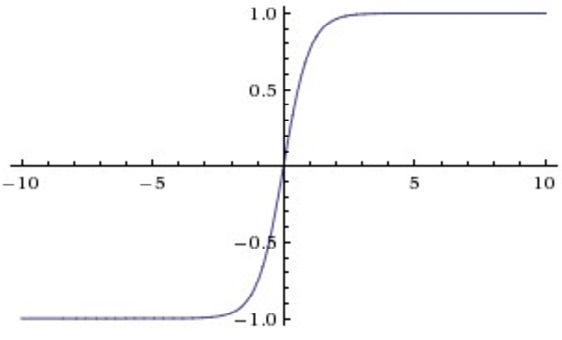
\includegraphics[width=\textwidth]{img/cnn/act_tanh.jpg}\\
Tanh activation\\
\\
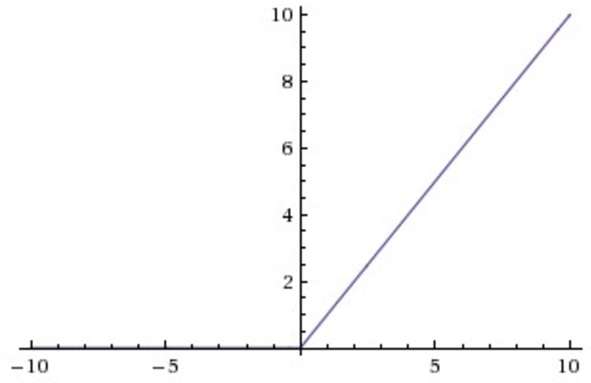
\includegraphics[width=\textwidth]{img/cnn/act_relu.jpg}\\
ReLu activation
\end{tabular}
\end{column}
\begin{column}{0.7\textwidth}
\textbf{Tanh} is a scaled sigmoid neuron: $tanh(x)=2\sigma(x)-1$. Differently to sigmoid, input is squashed in range [-1, 1], so the output is 0-centered. However, activation can still saturate and kill the gradient.\\
\vspace{0.5cm}
\textbf{ReLu} stands for Rectified Linear Unit and computes the function $f(x) = max(0, x)$. ReLu activation was found to greatly accelerate the convergence of SGD compared to sigmoid/tanh functions \cite{krizhevsky2012imagenet}. Furthermore, ReLu can be implemented by a simple threshold, \emph{w.r.t.} other activations which require complex operations.
\end{column}
\end{columns}
\end{frame}

%%%%%%%%%%%%%%%%%%%%%%%%%%%%%%%%%%%%%%%%%%%%%%%%%%%%%%%%%%%%%%%%%%

\begin{frame}{Neuron Activation}
\textbf{Why using non-linear activations at all?}\\
Composition of linear functions is a linear function. Without nonlinearities, neural networks would reduce to 1 layer logistic regression.\\
Let's say we have the following function ($\phi$ represent nonlinear activations):
\begin{equation*}
f(\bm{x}) = \phi(\mathbf{W_2}\phi(\mathbf{W_1x}))
\end{equation*}
If we get rid of nonlinearities, this reduces to:
\begin{equation*}
f(\bm{x}) = \mathbf{W_2}\mathbf{W_1x} = \bm{Wx} \quad where \quad \bm{W}=\bm{W_2W_1}
\end{equation*} 
which is clearly still linear.
\end{frame}

%%%%%%%%%%%%%%%%%%%%%%%%%%%%%%%%%%%%%%%%%%%%%%%%%%%%%%%%%%%%%%%%%%
%%%%%%%%%%%%%%%%%%%%%%%%%%%%%%%%%%%%%%%%%%%%%%%%%%%%%%%%%%%%%%%%%%
%%%%%%%%%%%%%%%%%%%%%%%%%%%%%%%%%%%%%%%%%%%%%%%%%%%%%%%%%%%%%%%%%%

\section{Neural Networks}

\begin{frame}{Neural Networks}
When we connect an ensemble of neurons in a graph is when the magic happens and we get an actual \textbf{neural network}.
\vspace{0.5cm}
\begin{columns}
\begin{column}{0.48\textwidth}
\centering
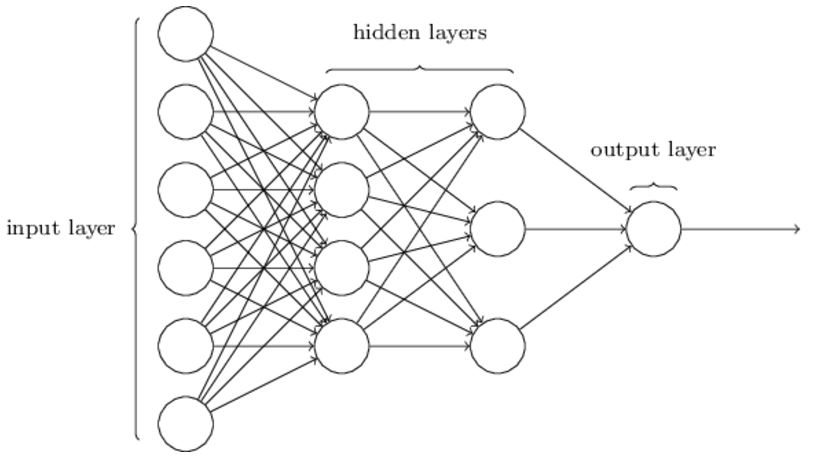
\includegraphics[width=1.0\textwidth]{img/dnn/neural_network.jpg}    \end{column}
\begin{column}{0.48\textwidth}
Neural networks are arranged in \textbf{layers}, with one \textit{input layer}, one \textit{output layer} and $N$ \textit{hidden layers} in the middle.\\
\vspace{0.5cm}
\textit{\small{The network depicted here has a total of $47$ learnable parameters. Does this make sense to you?}}
\end{column}
\end{columns}
\end{frame}

%%%%%%%%%%%%%%%%%%%%%%%%%%%%%%%%%%%%%%%%%%%%%%%%%%%%%%%%%%%%%%%%%%

\begin{frame}{Neural Networks}
The 4-layer network previously depicted can be simply expressed as:
\begin{equation}\label{eq:feedforward}
out = \phi(\mathbf{W_3}\phi(\mathbf{W_2}\phi(\mathbf{W_1x})))
\end{equation}
where:
\begin{columns}
\begin{column}{0.6\textwidth}
\begin{itemize}
\item $\phi$ is the activation function
\item $\mathbf{x} \in \R^{6}$ is the input 
\item $\mathbf{W_1} \in \R^{4x6}$ are the weights of first layer
\item $\mathbf{W_2} \in \R^{3x4}$ are the weights of second layer
\item $\mathbf{W_3} \in \R^{1x3}$ are the weights of third layer
\end{itemize}
\end{column}
\begin{column}{0.4\textwidth}
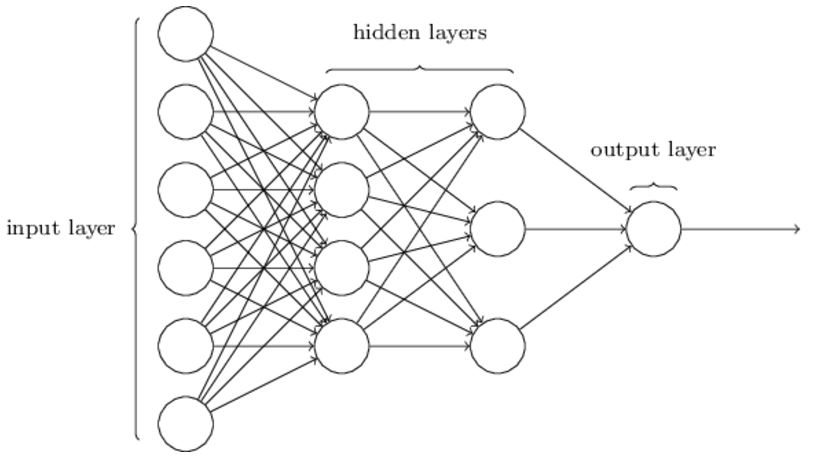
\includegraphics[width=0.8\textwidth]{img/dnn/neural_network.jpg}   
\end{column}
\end{columns}
\vspace{0.1cm}
\small{Notice that to ease the notation biases have been incorporated into weight matrices W.}
\end{frame}

%%%%%%%%%%%%%%%%%%%%%%%%%%%%%%%%%%%%%%%%%%%%%%%%%%%%%%%%%%%%%%%%%%

\begin{frame}{Forward propagation}

\textbf{Forward propagation} is the process of computing the network output given its input.
\begin{figure}
\begin{tabular}{c}
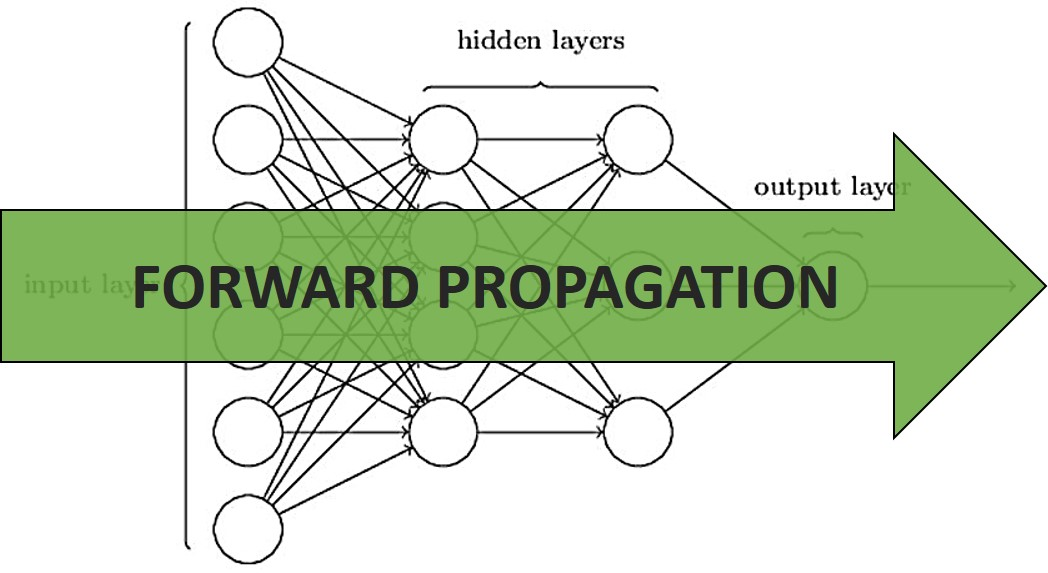
\includegraphics[width=0.5\textwidth]{img/dnn/forward_prop.jpg}
\end{tabular}
\end{figure}
The formula of forward propagation for our toy network above is the one in Eq. \ref{eq:feedforward}.

\end{frame}

%%%%%%%%%%%%%%%%%%%%%%%%%%%%%%%%%%%%%%%%%%%%%%%%%%%%%%%%%%%%%%%%%%

\begin{frame}{Representational Power}
It has been shown (\emph{e.g.} \cite{cybenko1989approximation}) that any continuous function $f(x)$ can be approximated at arbitrary precision $\epsilon > 0$ by a neural network $g(x)$ with at least one hidden layer.\\
That is:
\begin{equation*}
\forall x, \quad |f(x) - g(x)| < \epsilon
\end{equation*}
For this reason neural networks with at least one hidden layers are referred to as \textbf{universal approximators}.
In practice however networks with more layers often outperform 2-layer nets, despite the fact that on paper their representational power is equal.
\end{frame}

%%%%%%%%%%%%%%%%%%%%%%%%%%%%%%%%%%%%%%%%%%%%%%%%%%%%%%%%%%%%%%%%%%

\begin{frame}{Setting Hyperparameters}
The number of layers in the network, as well as the number of neurons in each layers, are so called \textbf{hyperparameters} of the architecture.\\
\vspace{0.25cm}
Keep in mind that:
\begin{itemize}
\item the bigger the size and the number of layers, the more the \textbf{capacity} of the network increases, which is good because the space of representable functions grow.\\
\item bigger networks without proper regularization are way more prone to \textbf{overfit} the training data, which is bad.
\end{itemize}

\end{frame}

%%%%%%%%%%%%%%%%%%%%%%%%%%%%%%%%%%%%%%%%%%%%%%%%%%%%%%%%%%%%%%%%%%

\begin{frame}{Setting Hyperparameters}
\begin{columns}
\begin{column}{0.6\textwidth}
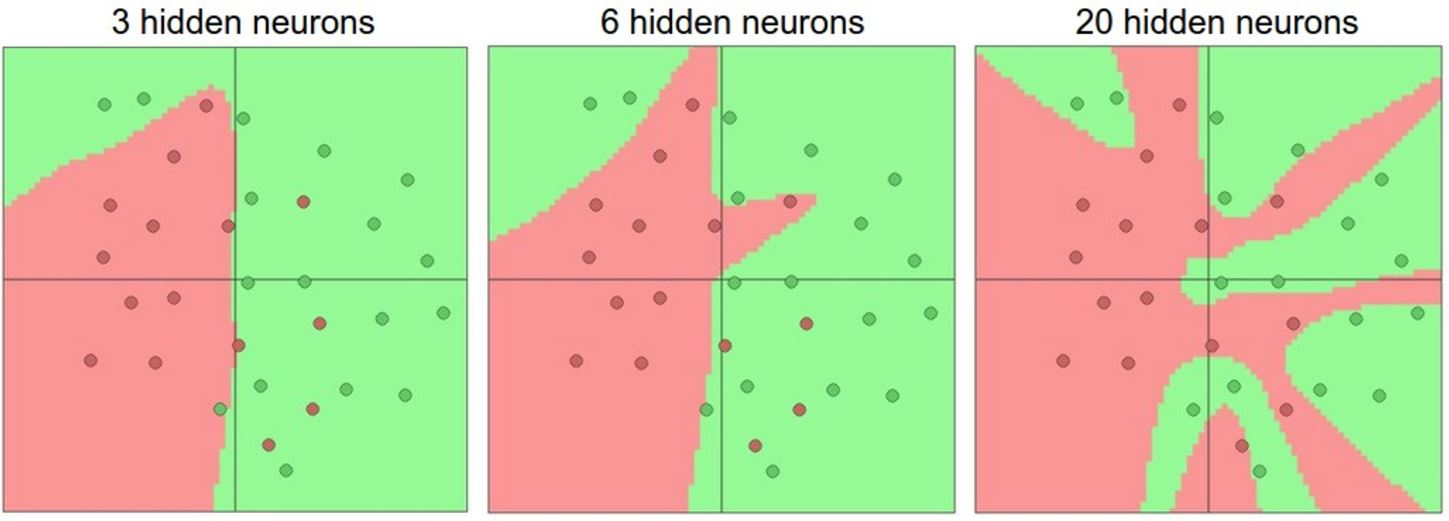
\includegraphics[width=0.9\textwidth]{img/dnn/dnn_overfit.jpg}\\
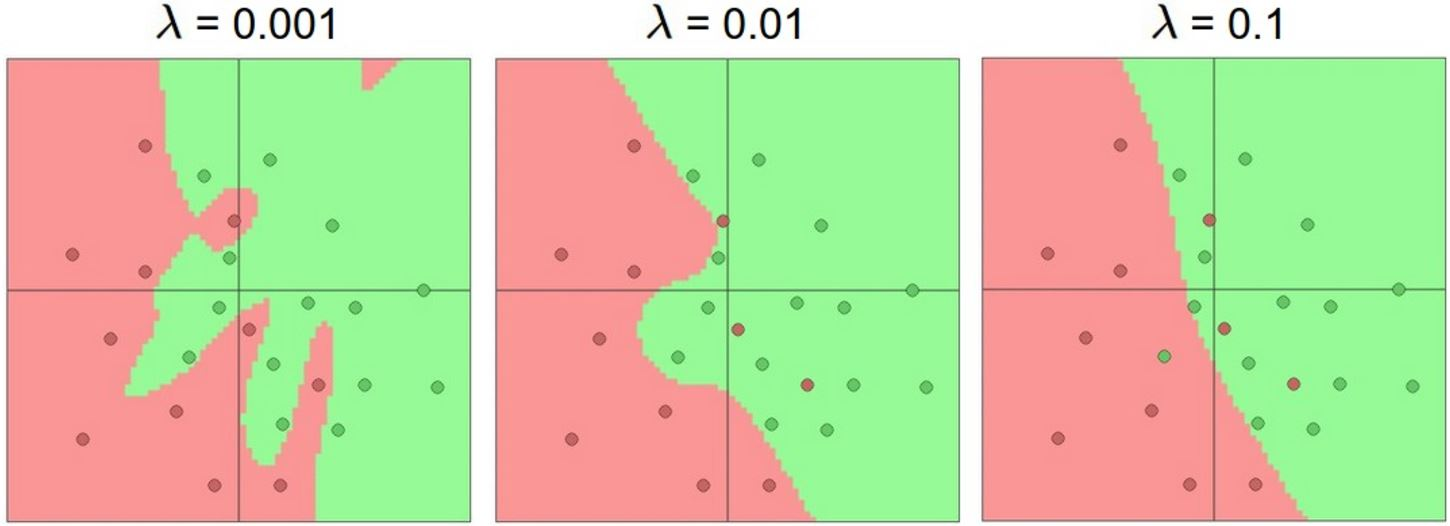
\includegraphics[width=0.9\textwidth]{img/dnn/dnn_overfit_reg.jpg}
\end{column}
\begin{column}{0.4\textwidth}
In practice, usually networks are made as big as computational budget allows.\\
\vspace{0.5cm}
Then overfitting is prevented through proper \textbf{regularization techniques} (\emph{e.g.} dropout, weights decay, input noise).
\end{column}
\end{columns}
\end{frame}

%%%%%%%%%%%%%%%%%%%%%%%%%%%%%%%%%%%%%%%%%%%%%%%%%%%%%%%%%%%%%%%%%%
%%%%%%%%%%%%%%%%%%%%%%%%%%%%%%%%%%%%%%%%%%%%%%%%%%%%%%%%%%%%%%%%%%
%%%%%%%%%%%%%%%%%%%%%%%%%%%%%%%%%%%%%%%%%%%%%%%%%%%%%%%%%%%%%%%%%%

\section{Training a DNN}


%%%%%%%%%%%%%%%%%%%%%%%%%%%%%%%%%%%%%%%%%%%%%%%%%%%%%%%%%%%%%%%%%%

\begin{frame}{Objective Function}

The \textbf{objective or loss function} \textbf{measures the quality of our mapping} from input to output. This function has a form of this kind:
\begin{equation*}
L(\bm{\theta}; \mathbf{x, y})=\frac{1}{N} \sum_i L_i(\bm{\theta}; \mathbf{x_i, y_i}) + \alpha \Omega (\bm{\theta})
\end{equation*}
where $N$ is the number of training examples, $\theta$ is the set of network parameters and $\alpha$ weights the regularization's strength.
In particular:
\begin{itemize}
\item The \emph{data term}, computed as an average over individual examples, measures the goodness of model's predictions \textit{w.r.t.} data labels. 
\item The \emph{regularization term} which depends only on network parameters and has the role to mitigate the risk of overfitting.
\end{itemize}
\end{frame}

%%%%%%%%%%%%%%%%%%%%%%%%%%%%%%%%%%%%%%%%%%%%%%%%%%%%%%%%%%%%%%%%%%

\begin{frame}{Objective Function}
The choice of the data loss depends on the task we want to solve.
\begin{itemize}
	\item \textbf{Classification}:
	\begin{itemize}
		\item \emph{hinge loss}:
		\begin{equation}
		L_i = \sum_{j\neq y_i}max(0, f_j - f_{y_i} + 1)
		\end{equation}
		\item \emph{softmax loss}:
		\begin{equation}
		L_i = -log\left(\frac{e^{f_{y_i}}}{\sum_j e^{f_j}}\right)
		\end{equation}
	\end{itemize}
	\item \textbf{Regression}:
	\begin{itemize}
		\item \emph{Mean Squared Error (MSE)}
		\begin{equation}
		L_i = || f - y_i ||^2_2
		\end{equation}
	\end{itemize}
\end{itemize}
These are just examples. The objective function is heavily task-dependent and is often customized to meet the specific problem constraints.
\end{frame}

%%%%%%%%%%%%%%%%%%%%%%%%%%%%%%%%%%%%%%%%%%%%%%%%%%%%%%%%%%%%%%%%%%


\begin{frame}{Learning the parameters}
During training phase, \textbf{we want to learn the set of network parameters which minimize the objective function} on the training set.\\
\vspace{0.5cm}
More formally:
\begin{equation*}
\bm{\theta}^* = argmin_{\theta} \left(\frac{1}{N} \sum_i L_i(\bm{\theta}; \mathbf{x_i, y_i}) + \alpha \Omega (\bm{\theta})\right)
\end{equation*}
\end{frame}

\begin{frame}{Backpropagation}
The algorithm used to compute the gradients of the loss functions with respect to its parameters is called \textbf{backpropagation}.\\
\vspace{0.5cm}
This procedure is based on \textit{chain rule of calculus}
\begin{equation*}
\frac{dz}{dx} = \frac{dz}{dy}\frac{dy}{dx} \quad where\ z = f(g(x)),\ y = g(x) 
\end{equation*}
and proceeds backwards \textit{w.r.t} the flow of computations performed to compute the loss itself (hence the name).

\end{frame}

%%%%%%%%%%%%%%%%%%%%%%%%%%%%%%%%%%%%%%%%%%%%%%%%%%%%%%%%%%%%%%%%%%

\begin{frame}{Backpropagation}
Backpropagation is a \textbf{local} process. Neurons are completely unaware of the complete topology of the network in which they are embedded.\\
\vspace{0.5cm}
Indeed, in order for backpropagation to work, \textbf{each neuron just need to be able to compute two things}:\\
\vspace{0.5cm}
\begin{columns}
\begin{column}{0.3\textwidth}
	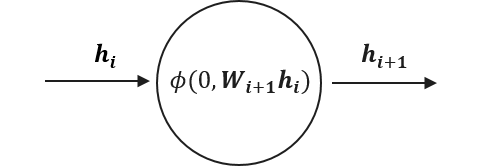
\includegraphics[width=\textwidth]{img/dnn/single_neuron_forward.png}
\end{column}
\begin{column}{0.7\textwidth}
	$\frac{\partial \bm{h_{i+1}}}{\partial \bm{W_{i+1}}}$ Derivative of its output with respect to its weights.\\
	\vspace{0.2cm}
	$\frac{\partial \bm{h_{i+1}}}{\partial \bm{h_{i}}}$ Derivative of its output with respect to its inputs.
\end{column}
\end{columns}
\vspace{0.5cm}
\end{frame}


%%%%%%%%%%%%%%%%%%%%%%%%%%%%%%%%%%%%%%%%%%%%%%%%%%%%%%%%%%%%%%%%%%

\begin{frame}{Backpropagation}
During backpropagation, the neuron will eventually discover the influence of its output value on the output of the whole network, that is will receive $\frac{\partial \bm{L}}{\partial \bm{h_{i+1}}}$.\\
\vspace{0.5cm}
\begin{figure}
\begin{tabular}{c}
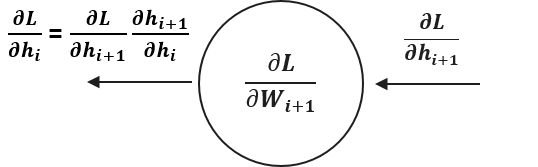
\includegraphics[width=0.5\textwidth]{img/dnn/single_neuron_backward.png}
\end{tabular}
\end{figure}
This gradient is then chained to local gradient and passed to previous neurons to continue the backpropagation flow.
\end{frame}

%%%%%%%%%%%%%%%%%%%%%%%%%%%%%%%%%%%%%%%%%%%%%%%%%%%%%%%%%%%%%%%%%%

\begin{frame}{Backpropagation: example}
\begin{tabular}{c}
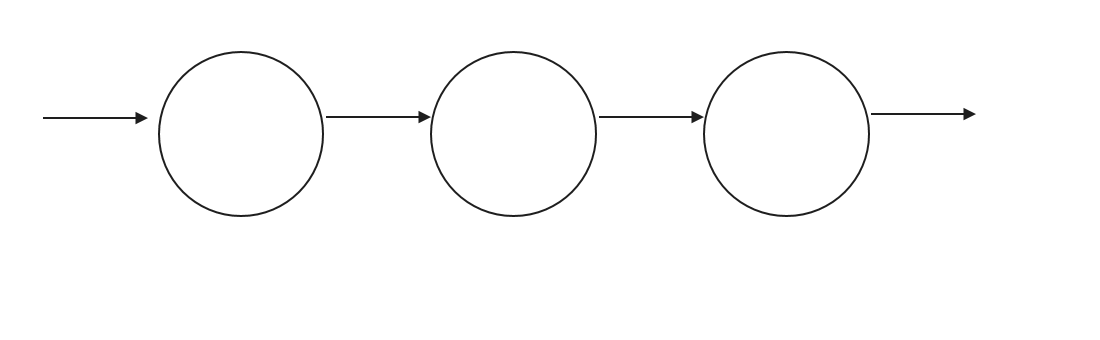
\includegraphics[width=1.\textwidth]{img/dnn/backprop/backprop_0.png}
\end{tabular}	
\end{frame}

%%%%%%%%%%%%%%%%%%%%%%%%%%%%%%%%%%%%%%%%%%%%%%%%%%%%%%%%%%%%%%%%%%

\begin{frame}{Backpropagation: example}
\begin{tabular}{c}
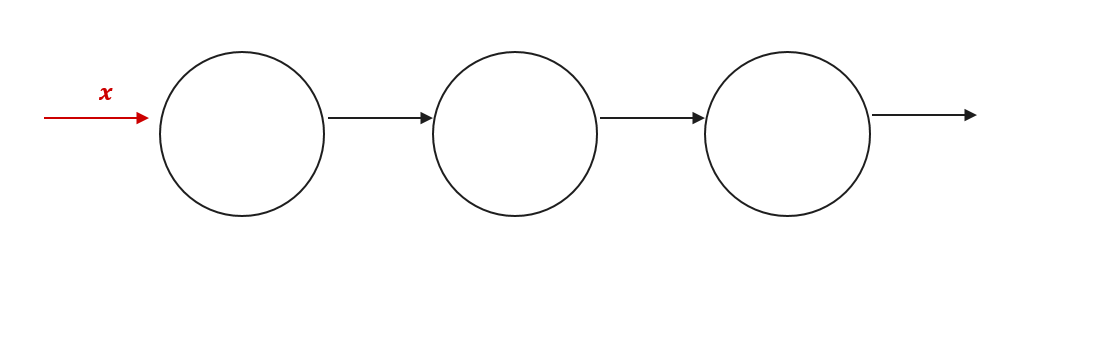
\includegraphics[width=1.\textwidth]{img/dnn/backprop/backprop_1.png}
\end{tabular}	
\end{frame}

%%%%%%%%%%%%%%%%%%%%%%%%%%%%%%%%%%%%%%%%%%%%%%%%%%%%%%%%%%%%%%%%%%

\begin{frame}{Backpropagation: example}
\begin{tabular}{c}
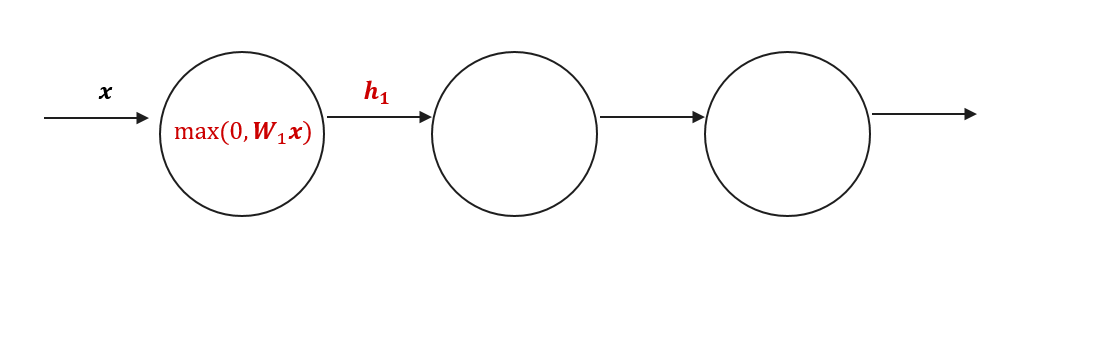
\includegraphics[width=1.\textwidth]{img/dnn/backprop/backprop_2.png}
\end{tabular}	
\end{frame}

%%%%%%%%%%%%%%%%%%%%%%%%%%%%%%%%%%%%%%%%%%%%%%%%%%%%%%%%%%%%%%%%%%

\begin{frame}{Backpropagation: example}
\begin{tabular}{c}
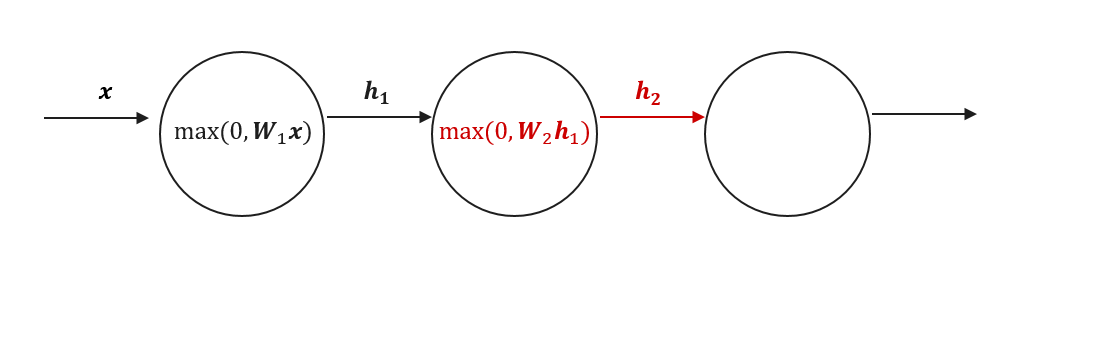
\includegraphics[width=1.\textwidth]{img/dnn/backprop/backprop_3.png}
\end{tabular}	
\end{frame}

%%%%%%%%%%%%%%%%%%%%%%%%%%%%%%%%%%%%%%%%%%%%%%%%%%%%%%%%%%%%%%%%%%

\begin{frame}{Backpropagation: example}
\begin{tabular}{c}
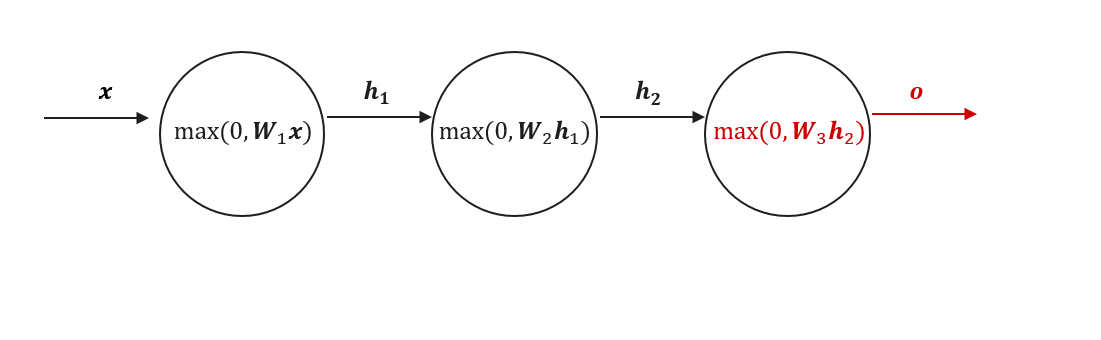
\includegraphics[width=1.\textwidth]{img/dnn/backprop/backprop_4.png}
\end{tabular}	
\end{frame}

%%%%%%%%%%%%%%%%%%%%%%%%%%%%%%%%%%%%%%%%%%%%%%%%%%%%%%%%%%%%%%%%%%

\begin{frame}{Backpropagation: example}
\begin{tabular}{c}
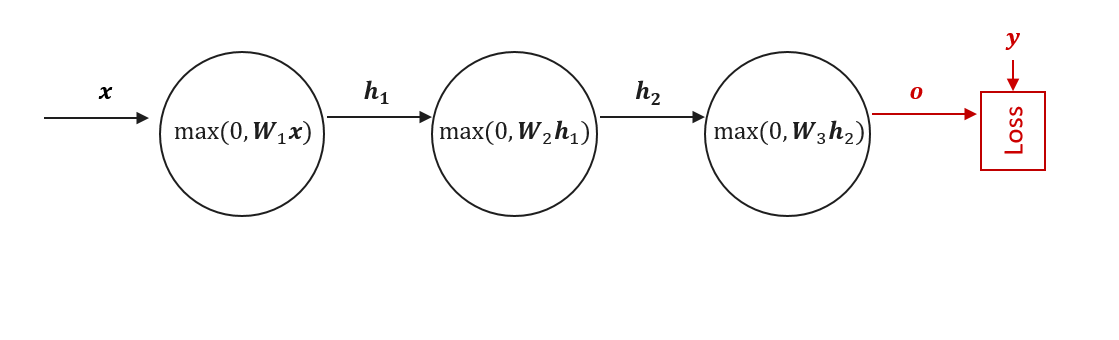
\includegraphics[width=1.\textwidth]{img/dnn/backprop/backprop_5.png}
\end{tabular}	
\end{frame}

%%%%%%%%%%%%%%%%%%%%%%%%%%%%%%%%%%%%%%%%%%%%%%%%%%%%%%%%%%%%%%%%%%

\begin{frame}{Backpropagation: example}
\begin{tabular}{c}
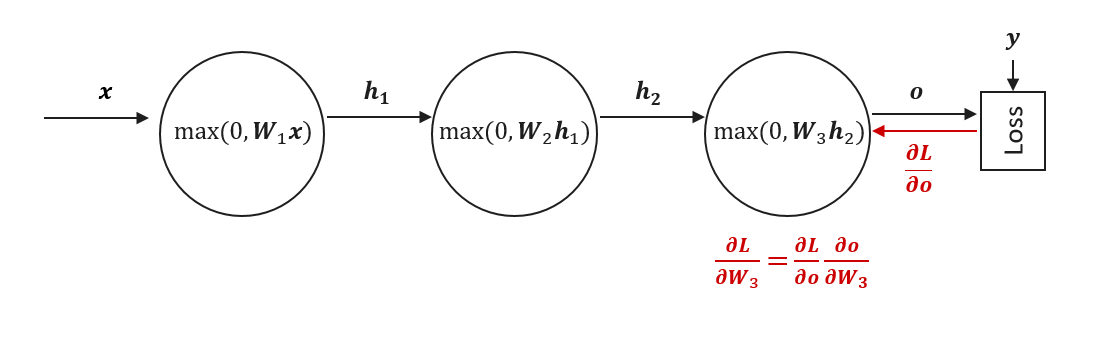
\includegraphics[width=1.\textwidth]{img/dnn/backprop/backprop_6.png}
\end{tabular}	
\end{frame}

%%%%%%%%%%%%%%%%%%%%%%%%%%%%%%%%%%%%%%%%%%%%%%%%%%%%%%%%%%%%%%%%%%

\begin{frame}{Backpropagation: example}
\begin{tabular}{c}
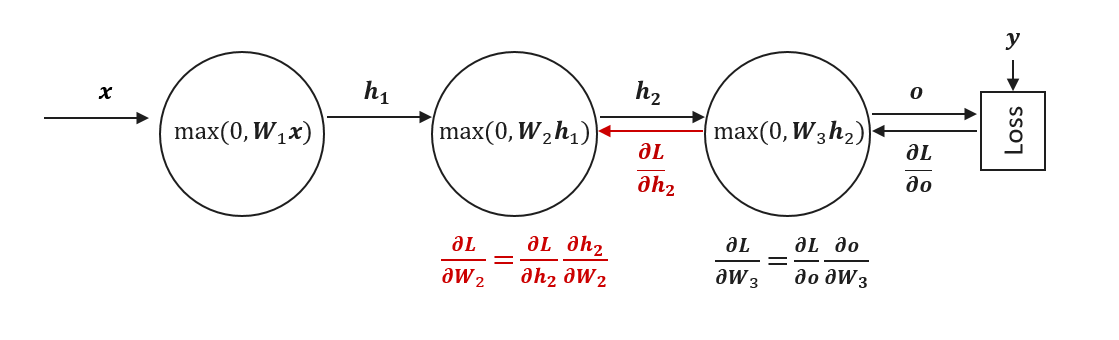
\includegraphics[width=1.\textwidth]{img/dnn/backprop/backprop_7.png}
\end{tabular}	
\end{frame}

%%%%%%%%%%%%%%%%%%%%%%%%%%%%%%%%%%%%%%%%%%%%%%%%%%%%%%%%%%%%%%%%%%

\begin{frame}{Backpropagation: example}
\begin{tabular}{c}
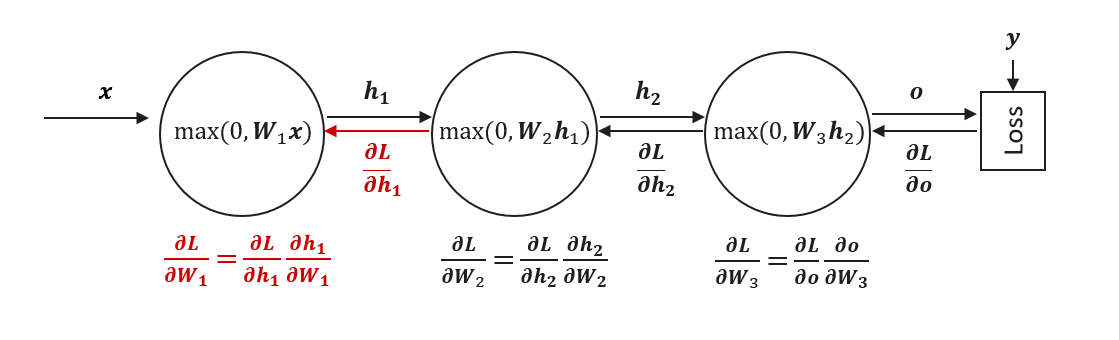
\includegraphics[width=1.\textwidth]{img/dnn/backprop/backprop_8.png}
\end{tabular}	
\end{frame}

%%%%%%%%%%%%%%%%%%%%%%%%%%%%%%%%%%%%%%%%%%%%%%%%%%%%%%%%%%%%%%%%%%

\begin{frame}{Weights Initialization}
When initializing the weights in the neural network, turns out that \textbf{random initialization} is very important to \textbf{break the symmetry}.\\
\vspace{0.2cm}
Indeed, if all weights were initialized to the same value (\emph{e.g.} $0$) then all neurons would compute the same output, the same gradient and would eventually undergo to the same update. Clearly, this is bad.\\
\vspace{0.2cm}
Common practice is to initialize all weights to small random numbers centered on zero (eventually scaled by neuron's \emph{fan-in} \cite{glorot2010understanding,he2015delving}) and all biases to zero.
\end{frame}

\begin{frame}{Dropout}
\vspace{0.5cm}
\begin{columns}
\begin{column}{0.3\textwidth}
\begin{tabular}{c}
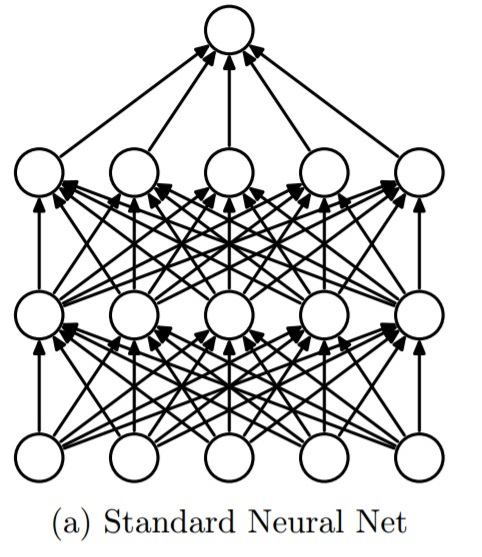
\includegraphics[width=0.65\textwidth]{img/dnn/dropout_no.jpg}\\
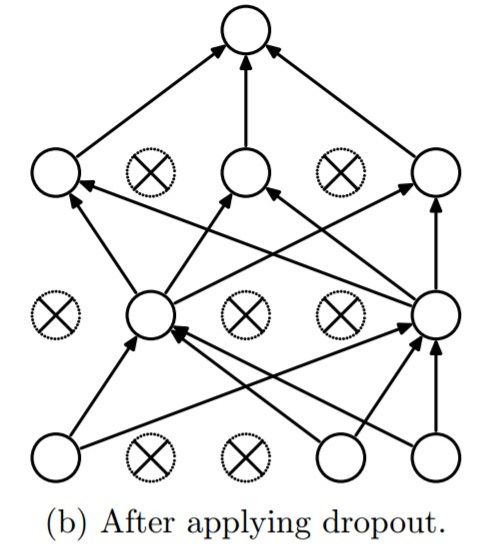
\includegraphics[width=0.65\textwidth]{img/dnn/dropout_yes.jpg}
\end{tabular}
\end{column}
\begin{column}{0.7\textwidth}
Besides traditional regularization techniques (\emph{e.g.} $L_n$ weight regularization), neural networks feature a simple and extremely effective regularization which is  \textbf{dropout}~\cite{srivastava2014dropout}.\\
\vspace{0.5cm}
During the training process, each neuron is set to zero (dropped) with a \emph{drop probability} $p$. This can be seen as sampling at each training step a different sub-network and updating only the corresponding portion of parameters.\\
\vspace{0.5cm}
At testing time, no dropout is applied. This can be interpreted as taking the average prediction of the ensemble of sub-networks.
\end{column}
\end{columns}
\end{frame}


%%%%%%%%%%%%%%%%%%%%%%%%%%%%%%%%%%%%%%%%%%%%%%%%%%%%%%%%%%%%%%%%%%
%%%%%%%%%%%%%%%%%%%%%%%%%%%%%%%%%%%%%%%%%%%%%%%%%%%%%%%%%%%%%%%%%%
%%%%%%%%%%%%%%%%%%%%%%%%%%%%%%%%%%%%%%%%%%%%%%%%%%%%%%%%%%%%%%%%%%

\section{Credits}
\begin{frame}{Credits}
These slides heavily borrow from the following Stanford course:
\begin{itemize}
\item \url{http://cs231n.stanford.edu/}
\end{itemize}
if you want to deepen your knowledge of these concepts, I'd really suggest to start from here!\\
\vspace{0.2cm}
Also, nice convolution animations are taken from here:
\begin{itemize}
\item \url{https://github.com/vdumoulin/conv_arithmetic}
\end{itemize}
\end{frame}

%%%%%%%%%%%%%%%%%%%%%%%%%%%%%%%%%%%%%%%%%%%%%%%%%%%%%%%%%%%%%%%%%%
%%%%%%%%%%%%%%%%%%%%%%%%%%%%%%%%%%%%%%%%%%%%%%%%%%%%%%%%%%%%%%%%%%
%%%%%%%%%%%%%%%%%%%%%%%%%%%%%%%%%%%%%%%%%%%%%%%%%%%%%%%%%%%%%%%%%%

\section{References}

\begin{frame}[t, allowframebreaks]
\frametitle{References}
\bibliographystyle{abbrv}
\bibliography{bibliography}
\end{frame}
\end{document}